% made with ♥ by Tekks
% allgem. Dokumentenformat
\documentclass[a4paper,12pt,headsepline]{scrartcl}
%Projektdaten
\newcommand{\projauthorvor}{Andreas}
\newcommand{\projauthornach}{Heil}
\newcommand{\projsubtitle}{Zweite Projektarbeit}
\newcommand{\arbeitstitel}{Konzeption und Entwicklung von Lernbausteinen im Themengebiet der Künstlichen Intelligenz mit dem Fokus auf die Anwendungsfelder Industrie 4.0 und Robotik}
%Hochschuldaten
\newcommand{\hochschule}{Duale Hochschule Baden-Württemberg Mosbach}
\newcommand{\matnr}{0000000}
\newcommand{\kurs}{WI16A}
\newcommand{\stg}{Wirtschaftsinformatik}
\newcommand{\stgprofil}{Industrie}
\newcommand{\zeitraum}{29.05. - 03.09.2017}
\newcommand{\stgleiter}{Prof. Dr. Christian Schalles}
%Betreuerdaten HS
\newcommand{\betreuer}{Reinhard Dietze}
\newcommand{\betreueremail}{RDie@gmx.net}
\newcommand{\betreuertelefon}{}
%Unternehmensdaten
\newcommand{\unt}{Unternehmensname}
\newcommand{\untanschr}{Stasse Nr  \\ & & PLZ Ort}
\newcommand{\untbetr}{Unt.Betreuer}
\newcommand{\emailbet}{Email Unt.Betreuer}
\newcommand{\telefonbet}{Tel.  Unt.Betreuer}

% weitere Pakete
% Grafiken aus PNG Dateien einbinden
\usepackage{graphicx}
\usepackage{xcolor}
% deutsche Silbentrennung
\usepackage[ngerman]{babel}
\overfullrule=0pt
% Eurozeichen einbinden
\usepackage[right]{eurosym}
% Grafikhauptverzeichnis
\graphicspath{{depictions/images/}}

% Zeichenencoding
\usepackage[T1]{fontenc}
\usepackage{mathptmx}
\usepackage{fix-cm}
\usepackage{fontspec}
\setmainfont[Path = subfiles/font/,BoldFont=timesbd.ttf,ItalicFont=timesi.ttf,BoldItalicFont=timesbi.ttf,]{times.ttf}

% floatende Bilder ermöglichen
\usepackage{float}

% mehrseitige Tabellen ermöglichen
\usepackage{longtable}

% Packet für Seitenrandabständex und Einstellung für Seitenränder
\usepackage{geometry}
\geometry{left=3cm, right=2.5cm, top=2.5cm, bottom=2.7cm}

% Paket für Boxen im Text
\usepackage{fancybox}
% bricht lange URLs "schoen" um
\usepackage[hyphens,obeyspaces,spaces]{url}
% Paket für Textfarben
\usepackage{color}

% Mathematische Symbole importieren
\usepackage{amssymb}

% erzeugt Inhaltsverzeichnis mit Querverweisen zu den Kapiteln (PDF Version)
\usepackage[bookmarksnumbered,pdftitle={\arbeitstitel},hyperfootnotes=false,pdfauthor={\projauthorvor \projauthornach}]{hyperref}
% Tiefe des Inhaltsverzeichnis
\setcounter{tocdepth}{7}
%\hypersetup{colorlinks, citecolor=red, linkcolor=blue, urlcolor=black}
%\hypersetup{colorlinks, citecolor=black, linkcolor= black, urlcolor=black}
% neue Kopfzeilen mit fancypaket
\usepackage{fancyhdr} %Paket laden
\pagestyle{fancy} %eigener Seitenstil
\fancyhf{} %alle Kopf- und Fußzeilenfelder bereinigen
\fancypagestyle{FooBar}{%
    \fancyhead{}
}
\fancyhead[L]{\nouppercase{\leftmark}} %Kopfzeile links
\fancyhead[C]{} %zentrierte Kopfzeile
%\fancyhead[R]{\thepage} %Kopfzeile rechts
\renewcommand{\headrulewidth}{0.3pt} %obere Trennlinie
\fancyfoot[L]{\footnotesize\projauthornach, \projauthorvor}
\fancyfoot[R]{\thepage}
\renewcommand{\footrulewidth}{0.4pt} %untere Trennlinie
\pagenumbering{gobble}
% für Tabellen
\usepackage{array}
\usepackage{csquotes}
% Runde Klammern für Zitate

\usepackage[backend=biber,%
            style=alphabetic,
            citestyle=alphabetic,
            maxalphanames=1,
            sorting=ynt,
            ]{biblatex}
\addbibresource{subfiles/bibfile.bib}
\renewcommand*{\labelalphaothers}{}
\DeclareLabelalphaTemplate{
  \labelelement{
    \field[final]{shorthand}
    \field{labelname}
    \field{label}
  }
  \labelelement{
    \literal{,\addhighpenspace}
  }
  \labelelement{
    \field{year}
  }
}

\renewcommand{\textcite}[2][]{\parentext{vgl. \cite[#1]{#2}}}
\renewcommand{\footcite}[2][]{\footnote{\parentext{vgl. \cite[#1]{#2}}}}
% Schaltet den zusätzlichen Zwischenraum ab, den LaTeX normalerweise nach einem Satzzeichen einfügt.
\frenchspacing

% Paket für Zeilenabstand
\usepackage{setspace}

% für Bildbezeichner
\usepackage{capt-of}

% für Stichwortverzeichnis
\usepackage{makeidx}

% für Listings
\usepackage{listings}

\definecolor{darkgreen}{RGB}{0,128,32}
\lstset{breaklines=true,
        tabsize=3,
        showstringspaces=false,
        numbers=left,
        xleftmargin=1cm,
        xrightmargin=1cm,
        aboveskip=1em,
        framexbottommargin=1pt,
        framextopmargin=1pt,
        captionpos=b,
        frame = single,}
\lstdefinestyle{Common}{extendedchars=\true, language={[Visual]Basic},morestring=[s]""}
\lstdefinestyle{C}{language=C++,
                basicstyle=\linespread{0.8}\ttfamily,
                keywordstyle=\color{blue}\ttfamily,
                stringstyle=\color{red}\ttfamily,
                commentstyle=\color{green}\ttfamily,
                morecomment=[l][\color{magenta}]{\#}}

% Indexerstellung
\makeindex

% Abkürzungsverzeichnis
\usepackage[german]{nomencl}
\let\abbrev\nomenclature

% Abkürzungsverzeichnis LiveTex Version
\renewcommand{\nomname}{Abkürzungsverzeichnis}
\setlength{\nomlabelwidth}{.25\hsize}
\renewcommand{\nomlabel}[1]{#1 \dotfill}
\setlength{\nomitemsep}{-\parsep}
\makenomenclature

\clubpenalty = 10000

\widowpenalty = 10000
\displaywidowpenalty = 10000

\begin{document}
% hier werden die Trennvorschläge inkludiert
%hier müssen alle Wörter rein, welche Latex von sich auch nicht korrekt trennt bzw. bei denen man die genaue Trennung vorgeben möchte
\hyphenation{
Film-pro-du-zen-ten
Lux-em-burg
Soft-ware-bau-steins
zeit-in-ten-siv
}

% Titelseite %
% das Papierformat zuerst
%\documentclass[a4paper, 11pt]{article}

% deutsche Silbentrennung
%\usepackage[ngerman]{babel}

% wegen deutschen Umlauten
%\usepackage[ansinew]{inputenc}

% hier beginnt das Dokument
%\begin{document}


\thispagestyle{empty}

\begin{figure}[t]
 \centering
 
\includegraphics[width=0.3\textwidth]{DHBWLogo}
~~~~~~~~~~~~~~~~~~~~~~~~~~~~~~~~~~~~~~~~~~~~
 
\includegraphics[width=0.4\textwidth]{CompanyLogo}
\end{figure}

\begin{verbatim}
\end{verbatim}

\begin{center}
\hochschule \\[1ex]
\projsubtitle
\end{center}

\begin{verbatim}
\end{verbatim}

\begin{center}
\doublespacing
\textbf{\LARGE{\arbeitstitel}}\\
\singlespacing
\begin{verbatim}
\end{verbatim}
Verfasser: 
\textbf{\projauthorvor~\projauthornach}
\end{center}

\begin{verbatim}

\end{verbatim}
\begin{center}
Studiengang \stg \\Profil: \stgprofil \\Zeitraum: \zeitraum
\end{center}

\begin{verbatim}
\end{verbatim}

\begin{flushleft}
\begin{tabular}{llll}
\textbf{Matrikelnummer:} & & \matnr & \\
\textbf{Kurs:} & & \kurs & \\
& & \\
\textbf{Hochschule:} & & \hochschule &\\
\textbf{Studiengangsleiter:} & & \stgleiter &\\
\textbf{Wissenschaftlicher Betreuer:} & & \betreuer &\\
\textbf{E-Mail:} & & \betreueremail &\\
& & \\
\textbf{Ausbildungsunternehmen:} & & \unt \\ & & \untanschr \\
\textbf{Unternehmensbetreuer:} & & \untbetr& \\
\textbf{Telefon:} & & \telefonbet& \\
\textbf{E-Mail:} & & \emailbet& \\
\end{tabular}
\end{flushleft}
\begin{verbatim}

\end{verbatim}
\begin{center}
Sperrvermerk
\end{center}


% 1.5 facher Zeilenabstand
\onehalfspacing

% Sperrvermerk
\section*{Sperrvermerk}
Die vorliegende Arbeit beinhaltet vertrauliche Informationen der Firma \unt. Sie ist nur für die Beteiligten am Begutachtungs- und Evaluationsprozess bestimmt.\\Die Weitergabe des Inhalts der Arbeit im Ganzen oder von Teilen daraus an externe Dritte sowie das Anfertigen von Abschriften oder Kopien zu welchem Zweck, in welcher Form und zu welchem Zeitpunkt auch immer sind grundsätzlich untersagt. Ausnahmen bedürfen der schriftlichen Genehmigung der Firma \unt.\\Eine Weitergabe an Mitarbeiter der Hochschule aufgrund fachlicher Belange oder für administrative Zwecke ist von dieser Regelung explizit ausgenommen.

% Einleitung / Abstract
\section*{Zusammenfassung}
Lorem ipsum dolor sit amet, consectetur adipiscing elit, sed do eiusmod tempor incididunt ut labore et dolore magna aliqua. Sed odio morbi quis commodo odio aenean. Eleifend quam adipiscing vitae proin sagittis nisl rhoncus. Habitant morbi tristique senectus et netus et malesuada. Est ultricies integer quis auctor elit sed. At erat pellentesque adipiscing commodo elit at imperdiet dui accumsan. Interdum posuere lorem ipsum dolor.
\newpage
\section*{Abstract}
Lorem ipsum dolor sit amet, consectetur adipiscing elit, sed do eiusmod tempor incididunt ut labore et dolore magna aliqua. Sed odio morbi quis commodo odio aenean. Eleifend quam adipiscing vitae proin sagittis nisl rhoncus. Habitant morbi tristique senectus et netus et malesuada. Est ultricies integer quis auctor elit sed. At erat pellentesque adipiscing commodo elit at imperdiet dui accumsan. Interdum posuere lorem ipsum dolor.
\newpage

\singlespacing

% Inhaltsverzeichnis anzeigen
\pagenumbering {roman}
\newpage
\fancyhead[L]{Inhaltsverzeichnis}\thispagestyle{FooBar}
\tableofcontents

% das Abbildungsverzeichnis
\newpage
% Abbildungsverzeichnis soll im Inhaltsverzeichnis auftauchen
\addcontentsline{toc}{section}{Abbildungsverzeichnis}\thispagestyle{FooBar}
\listoffigures
\newpage
\addcontentsline{toc}{section}{Tabellenverzeichnis}\thispagestyle{FooBar}
\listoftables
\newpage
\addcontentsline{toc}{section}{Listingverzeichnis}\thispagestyle{FooBar}
\renewcommand{\lstlistlistingname}{Listingverzeichnis}
% Verzeichnisse sollen im Inhaltsverzeichnis auftauchen
\lstlistoflistings

\newcommand{\au}{\glqq}
\newcommand{\ao}{\grqq}
% das Abkürzungsverzeichnis
\newpage
\fancyhead[L]{Abkürzungsverzeichnis} %Kopfzeile links
%Abkürzungen
\nomenclature{SMA}{Smart MES Applications}
\nomenclature{DM}{Data Mining}
\nomenclature{DHBW}{Duale Hochschule Baden-Württemberg}
\nomenclature{KNN}{Künstliche neuronale Netze}
\nomenclature{BT}{Brain Technologie}
\nomenclature{KI}{Künstliche Intelligenz}

\printnomenclature
\addcontentsline{toc}{section}{Abkürzungsverzeichnis}\thispagestyle{FooBar}

\setlength{\columnsep}{25pt}

%%%%%%% EINLEITUNG %%%%%%%%%%%%

\newpage
\onehalfspacing
\pagenumbering {arabic}
\fancyhead[L]{\nouppercase{\leftmark}}

\section{Einleitung}\label{einleitung}\thispagestyle{FooBar}
\subsection{Gegenstand der Arbeit}
\begin{itshape}\au Nicht alles was zählt, kann gezählt werden, und nicht alles was gezählt werden
kann, zählt!\ao\end{itshape}  \citeboo[vgl.][S.29]{Wintson.2017}
\\\\
Lorem ipsum dolor sit amet, consectetur adipiscing elit, sed do eiusmod tempor incididunt ut labore et dolore magna aliqua. Nullam non nisi est sit amet facilisis. Sit amet nisl suscipit adipiscing bibendum est ultricies integer. Lorem ipsum dolor sit amet consectetur adipiscing elit duis. Morbi blandit cursus risus at ultrices mi.
\\
Lorem ipsum dolor sit amet, consectetur adipiscing elit, sed do eiusmod tempor incididunt ut labore et dolore magna aliqua. Nullam non nisi est sit amet facilisis. Sit amet nisl suscipit adipiscing bibendum est ultricies integer. Lorem ipsum dolor sit amet consectetur adipiscing elit duis. Morbi blandit cursus risus at ultrices mi.
\subsection{Zielsetzung der Arbeit}
Lorem ipsum dolor sit amet, consectetur adipiscing elit, sed do eiusmod tempor incididunt ut labore et dolore magna aliqua. Nullam non nisi est sit amet facilisis. Sit amet nisl suscipit adipiscing bibendum est ultricies integer. Lorem ipsum dolor sit amet consectetur adipiscing elit duis. Morbi blandit cursus risus at ultrices mi.
\subsection{Aufbau der Arbeit}
Lorem ipsum dolor sit amet, consectetur adipiscing elit, sed do eiusmod tempor incididunt ut labore et dolore magna aliqua. Non enim praesent elementum facilisis leo vel fringilla est. Bibendum enim facilisis gravida neque convallis a cras. Quam nulla porttitor massa id neque aliquam vestibulum morbi blandit. Gravida arcu ac tortor dignissim convallis aenean. Leo in vitae turpis massa sed elementum. Laoreet suspendisse interdum consectetur libero id faucibus nisl tincidunt. Mus mauris vitae ultricies leo integer. Rutrum tellus pellentesque eu tincidunt tortor aliquam nulla facilisi. Lectus mauris ultrices eros in cursus turpis. Dui nunc mattis enim ut tellus. Neque ornare aenean euismod elementum nisi quis. Diam sollicitudin tempor id eu nisl. Dolor sit amet consectetur adipiscing elit duis tristique. Metus aliquam eleifend mi in nulla posuere.
\subsection{Aufbau der Arbeit}
Lorem ipsum dolor sit amet, consectetur adipiscing elit, sed do eiusmod tempor incididunt ut labore et dolore magna aliqua. Non enim praesent elementum facilisis leo vel fringilla est. Bibendum enim facilisis gravida neque convallis a cras. Quam nulla porttitor massa id neque aliquam vestibulum morbi blandit. Gravida arcu ac tortor dignissim convallis aenean. Leo in vitae turpis massa sed elementum. Laoreet suspendisse interdum consectetur libero id faucibus nisl tincidunt. Mus mauris vitae ultricies leo integer. Rutrum tellus pellentesque eu tincidunt tortor aliquam nulla facilisi. Lectus mauris ultrices eros in cursus turpis. Dui nunc mattis enim ut tellus. Neque ornare aenean euismod elementum nisi quis. Diam sollicitudin tempor id eu nisl. Dolor sit amet consectetur adipiscing elit duis tristique. Metus aliquam eleifend mi in nulla posuere.
\newpage

\section{Theoretische Grundlagen}\label{theoretische_grundlagen}\thispagestyle{FooBar}
\subsection{Lorem}
Lorem ipsum dolor sit amet, consectetur adipiscing elit, sed do eiusmod tempor incididunt ut labore et dolore magna aliqua. Nullam non nisi est sit amet facilisis. Sit amet nisl suscipit adipiscing bibendum est ultricies integer. Lorem ipsum dolor sit amet consectetur adipiscing elit duis. Morbi blandit cursus risus at ultrices mi.  \footcite[10]{Vogel.2005}
\subsubsection{Lorem}
Lorem ipsum dolor sit amet, consectetur adipiscing elit, sed do eiusmod tempor incididunt ut labore et dolore magna aliqua. Nullam non nisi est sit amet facilisis. Sit amet nisl suscipit adipiscing bibendum est ultricies integer. Lorem ipsum dolor sit amet consectetur adipiscing elit duis. Morbi blandit cursus risus at ultrices mi. \textcite[10]{Vogel.2005}
\subsubsection{Lorem}
Lorem ipsum dolor sit amet, consectetur adipiscing elit, sed do eiusmod tempor incididunt ut labore et dolore magna aliqua. Nullam non nisi est sit amet facilisis. Sit amet nisl suscipit adipiscing bibendum est ultricies integer. Lorem ipsum dolor sit amet consectetur adipiscing elit duis. Morbi blandit cursus risus at ultrices mi.
\subsubsection{Lorem}
Lorem ipsum dolor sit amet, consectetur adipiscing elit, sed do eiusmod tempor incididunt ut labore et dolore magna aliqua. Nullam non nisi est sit amet facilisis. Sit amet nisl suscipit adipiscing bibendum est ultricies integer. Lorem ipsum dolor sit amet consectetur adipiscing elit duis. Morbi blandit cursus risus at ultrices mi. 
\newpage
\subsection{Lorem}
Lorem ipsum dolor sit amet consectetur adipiscing elit duis. Morbi blandit cursus risus at ultrices mi.Lorem ipsum dolor sit amet consectetur adipiscing elit duis. Morbi blandit cursus risus at ultrices mi.Lorem ipsum dolor sit amet consectetur adipiscing elit duis. Morbi blandit cursus risus at ultrices mi.
\subsubsection{Lorem}
Lorem ipsum dolor sit amet consectetur adipiscing elit duis. Morbi blandit cursus risus at ultrices mi.Lorem ipsum dolor sit amet consectetur adipiscing elit duis. Morbi blandit cursus risus at ultrices mi.Lorem ipsum dolor sit amet consectetur adipiscing elit duis. Morbi blandit cursus risus at ultrices mi.Lorem ipsum dolor sit amet consectetur adipiscing elit duis. Morbi blandit cursus risus at ultrices mi.
\subsubsection{Lorem}
\begin{figure}[h]
 \centering
 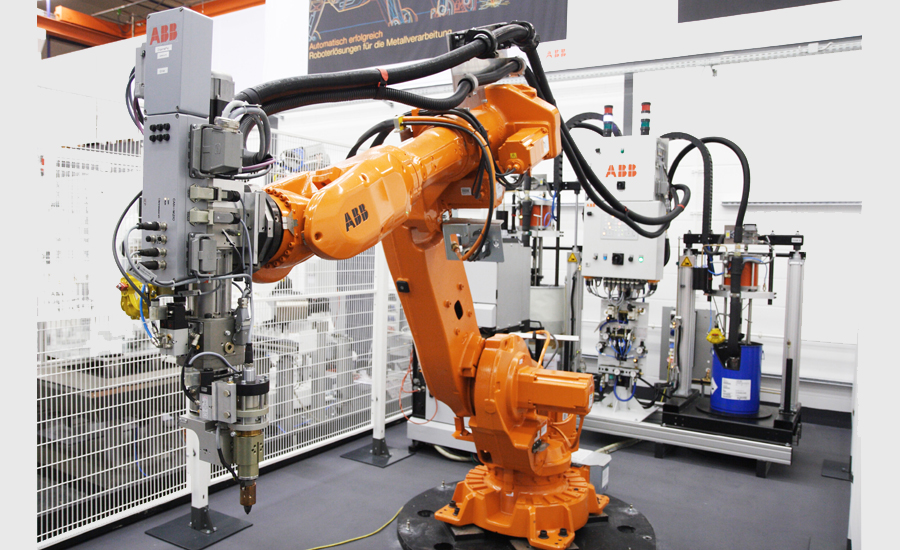
\includegraphics[width=0.8\textwidth,angle=0]{robot}
 \caption[Robot]{Robot}\label{fig:Robot}
\end{figure}
\newpage

\fancyhead[L]{\nouppercase{}} 
\section{Rahmenbedingungen}\label{rahmenbedingungen}
\subsection{Lorem}
\subsection{Lorem}
Lorem ipsum dolor sit amet, consectetur adipiscing elit, sed do eiusmod tempor incididunt ut labore et dolore magna aliqua. Integer eget aliquet nibh praesent tristique magna. Amet justo donec enim diam vulputate ut pharetra sit amet. Placerat duis ultricies lacus sed turpis tincidunt. Viverra mauris in aliquam sem fringilla. Enim diam vulputate ut pharetra sit amet. Fermentum odio eu feugiat pretium. Vestibulum lectus mauris ultrices eros in cursus. Purus sit amet volutpat consequat mauris nunc congue nisi. Sapien faucibus et molestie ac feugiat sed lectus vestibulum. Mattis ullamcorper velit sed ullamcorper morbi tincidunt ornare massa eget.
\subsubsection{Lorem}
Habitasse platea dictumst vestibulum rhoncus. Integer enim neque volutpat ac tincidunt vitae semper quis. Lectus vestibulum mattis ullamcorper velit sed. Fermentum et sollicitudin ac orci phasellus. Fringilla est ullamcorper eget nulla facilisi etiam dignissim. Turpis egestas sed tempus urna et pharetra pharetra massa. Posuere urna nec tincidunt praesent semper feugiat nibh sed pulvinar. Aliquet bibendum enim facilisis gravida. A diam maecenas sed enim ut. Sit amet consectetur adipiscing elit duis. Adipiscing bibendum est ultricies integer quis auctor elit sed.
\subsubsection{Lorem}
Tortor dignissim convallis aenean et tortor at risus viverra adipiscing. Suspendisse sed nisi lacus sed viverra tellus. Tempor orci dapibus ultrices in iaculis nunc sed. Nisi vitae suscipit tellus mauris a diam. Morbi tincidunt augue interdum velit euismod. Nunc vel risus commodo viverra maecenas accumsan lacus. Ullamcorper sit amet risus nullam eget felis eget nunc lobortis. Quisque id diam vel quam elementum pulvinar etiam. In hendrerit gravida rutrum quisque non tellus orci. Ut etiam sit amet nisl purus. Sit amet massa vitae tortor. Id interdum velit laoreet id donec ultrices tincidunt arcu. Quam adipiscing vitae proin sagittis nisl rhoncus mattis rhoncus urna. Faucibus in ornare quam viverra orci. Orci dapibus ultrices in iaculis. Pellentesque eu tincidunt tortor aliquam nulla facilisi. Lacus luctus accumsan tortor posuere ac ut. Ut ornare lectus sit amet est placerat in.
\subsection{Lorem}
Tincidunt augue interdum velit euismod. Sagittis purus sit amet volutpat consequat. Ut porttitor leo a diam sollicitudin tempor. Pellentesque habitant morbi tristique senectus et netus et malesuada fames. Quam id leo in vitae turpis massa sed. Erat velit scelerisque in dictum non consectetur a. Volutpat blandit aliquam etiam erat velit scelerisque. At augue eget arcu dictum varius duis at consectetur. Enim nulla aliquet porttitor lacus luctus accumsan tortor. Integer quis auctor elit sed vulputate mi sit amet. Habitant morbi tristique senectus et netus et malesuada. Vestibulum sed arcu non odio euismod lacinia. Semper eget duis at tellus at urna condimentum. Phasellus egestas tellus rutrum tellus pellentesque. Blandit cursus risus at ultrices mi tempus imperdiet nulla malesuada. Praesent semper feugiat nibh sed. Malesuada nunc vel risus commodo viverra maecenas accumsan. Risus nec feugiat in fermentum posuere urna nec tincidunt praesent. Mauris sit amet massa vitae tortor.
\lstinputlisting[style=C,caption={Codesnip},label={Codesnip}]{files/code/code1.c}
\subsection{Lorem}
Nec ultrices dui sapien eget mi proin sed libero enim. Semper risus in hendrerit gravida rutrum quisque. Fringilla urna porttitor rhoncus dolor. Malesuada fames ac turpis egestas. Velit scelerisque in dictum non. Imperdiet proin fermentum leo vel orci porta non pulvinar neque. Proin sed libero enim sed faucibus turpis in. Arcu non odio euismod lacinia at. Vestibulum lorem sed risus ultricies tristique nulla aliquet. Fames ac turpis egestas maecenas pharetra convallis posuere. Rutrum quisque non tellus orci ac auctor augue. Ornare arcu dui vivamus arcu. Morbi enim nunc faucibus a pellentesque. Felis eget velit aliquet sagittis id consectetur purus ut. Suspendisse in est ante in nibh. Eleifend quam adipiscing vitae proin sagittis nisl. Euismod elementum nisi quis eleifend quam adipiscing vitae proin sagittis.
\begin{table}[h]
 \centering
 \begin{tabular}{|c|c|}\hline
   4 & Anzahl Tage pro Woche \\ \hline
   1 & Anzahl der Wochen am Stück \\ \hline
   5 & Anzahl der Mitarbeiter \\ \hline
   Auswertung\_src & Zielblatt \\ \hline
   G25 & Zielrange auf Zielblatt \\ \hline
 \end{tabular}
 \caption{Tabelle}\label{fig:tabelle}
\end{table}
\newpage

\section{Lorem}\label{kennzahlenauswertung}\thispagestyle{FooBar}
\subsection{Lorem}
Lorem ipsum dolor sit amet, consectetur adipiscing elit, sed do eiusmod tempor incididunt ut labore et dolore magna aliqua. Integer eget aliquet nibh praesent tristique magna. Amet justo donec enim diam vulputate ut pharetra sit amet. Placerat duis ultricies lacus sed turpis tincidunt. Viverra mauris in aliquam sem fringilla. Enim diam vulputate ut pharetra sit amet. Fermentum odio eu feugiat pretium. Vestibulum lectus mauris ultrices eros in cursus. Purus sit amet volutpat consequat mauris nunc congue nisi. Sapien faucibus et molestie ac feugiat sed lectus vestibulum. Mattis ullamcorper velit sed ullamcorper morbi tincidunt ornare massa eget.
\subsection{Lorem}
Habitasse platea dictumst vestibulum rhoncus. Integer enim neque volutpat ac tincidunt vitae semper quis. Lectus vestibulum mattis ullamcorper velit sed. Fermentum et sollicitudin ac orci phasellus. Fringilla est ullamcorper eget nulla facilisi etiam dignissim. Turpis egestas sed tempus urna et pharetra pharetra massa. Posuere urna nec tincidunt praesent semper feugiat nibh sed pulvinar. Aliquet bibendum enim facilisis gravida. A diam maecenas sed enim ut. Sit amet consectetur adipiscing elit duis. Adipiscing bibendum est ultricies integer quis auctor elit sed.
\subsection{Lorem}
Tortor dignissim convallis aenean et tortor at risus viverra adipiscing. Suspendisse sed nisi lacus sed viverra tellus. Tempor orci dapibus ultrices in iaculis nunc sed. Nisi vitae suscipit tellus mauris a diam. Morbi tincidunt augue interdum velit euismod. Nunc vel risus commodo viverra maecenas accumsan lacus. Ullamcorper sit amet risus nullam eget felis eget nunc lobortis. Quisque id diam vel quam elementum pulvinar etiam. In hendrerit gravida rutrum quisque non tellus orci. Ut etiam sit amet nisl purus. Sit amet massa vitae tortor. Id interdum velit laoreet id donec ultrices tincidunt arcu. Quam adipiscing vitae proin sagittis nisl rhoncus mattis rhoncus urna. Faucibus in ornare quam viverra orci. Orci dapibus ultrices in iaculis. Pellentesque eu tincidunt tortor aliquam nulla facilisi. Lacus luctus accumsan tortor posuere ac ut. Ut ornare lectus sit amet est placerat in.
\subsection{Lorem}
Tincidunt augue interdum velit euismod. Sagittis purus sit amet volutpat consequat. Ut porttitor leo a diam sollicitudin tempor. Pellentesque habitant morbi tristique senectus et netus et malesuada fames. Quam id leo in vitae turpis massa sed. Erat velit scelerisque in dictum non consectetur a. Volutpat blandit aliquam etiam erat velit scelerisque. At augue eget arcu dictum varius duis at consectetur. Enim nulla aliquet porttitor lacus luctus accumsan tortor. Integer quis auctor elit sed vulputate mi sit amet. Habitant morbi tristique senectus et netus et malesuada. Vestibulum sed arcu non odio euismod lacinia. Semper eget duis at tellus at urna condimentum. Phasellus egestas tellus rutrum tellus pellentesque. Blandit cursus risus at ultrices mi tempus imperdiet nulla malesuada. Praesent semper feugiat nibh sed. Malesuada nunc vel risus commodo viverra maecenas accumsan. Risus nec feugiat in fermentum posuere urna nec tincidunt praesent. Mauris sit amet massa vitae tortor.
\subsubsection{Lorem}
Nec ultrices dui sapien eget mi proin sed libero enim. Semper risus in hendrerit gravida rutrum quisque. Fringilla urna porttitor rhoncus dolor. Malesuada fames ac turpis egestas. Velit scelerisque in dictum non. Imperdiet proin fermentum leo vel orci porta non pulvinar neque. Proin sed libero enim sed faucibus turpis in. Arcu non odio euismod lacinia at. Vestibulum lorem sed risus ultricies tristique nulla aliquet. Fames ac turpis egestas maecenas pharetra convallis posuere. Rutrum quisque non tellus orci ac auctor augue. Ornare arcu dui vivamus arcu. Morbi enim nunc faucibus a pellentesque. Felis eget velit aliquet sagittis id consectetur purus ut. Suspendisse in est ante in nibh. Eleifend quam adipiscing vitae proin sagittis nisl. Euismod elementum nisi quis eleifend quam adipiscing vitae proin sagittis.
\newpage

\section{Schlussbemerkung}\label{schlussbemerkung}\thispagestyle{FooBar}
\subsection{Lorem}
Lorem ipsum dolor sit amet, consectetur adipiscing elit, sed do eiusmod tempor incididunt ut labore et dolore magna aliqua. Nullam non nisi est sit amet facilisis. Sit amet nisl suscipit adipiscing bibendum est ultricies integer. Lorem ipsum dolor sit amet consectetur adipiscing elit duis. Morbi blandit cursus risus at ultrices mi.Lorem ipsum dolor sit amet, consectetur adipiscing elit, sed do eiusmod tempor incididunt ut labore et dolore magna aliqua. Nullam non nisi est sit amet facilisis. Sit amet nisl suscipit adipiscing bibendum est ultricies integer. Lorem ipsum dolor sit amet consectetur adipiscing elit duis. Morbi blandit cursus risus at ultrices mi.
\subsection{Lorem}
Lorem ipsum dolor sit amet, consectetur adipiscing elit, sed do eiusmod tempor incididunt ut labore et dolore magna aliqua Kapitel~\ref{rahmenbedingungen} Lorem ipsum dolor sit amet, consectetur adipiscing elit, sed do eiusmod tempor incididunt ut labore et dolore magna aliqua.
\begin{itemize}
\item Lorem ipsum dolor sit amet, consectetur adipiscing elit, sed do eiusmod tempor incididunt ut labore et dolore magna aliqua.
\item Lorem ipsum dolor sit amet, consectetur adipiscing elit, sed do eiusmod tempor incididunt ut labore et dolore magna aliqua.
\item Lorem ipsum dolor sit amet, consectetur adipiscing elit, sed do eiusmod tempor incididunt ut labore et dolore magna aliqua.
\item Lorem ipsum dolor sit amet, consectetur adipiscing elit, sed do eiusmod tempor incididunt ut labore et dolore magna aliqua.
\item Lorem ipsum dolor sit amet, consectetur adipiscing elit, sed do eiusmod tempor incididunt ut labore et dolore magna aliqua.
\end{itemize}
Lorem ipsum dolor sit amet, consectetur adipiscing elit, sed do eiusmod tempor incididunt ut labore et dolore magna aliqua. Nullam non nisi est sit amet facilisis. Sit amet nisl suscipit adipiscing bibendum est ultricies integer. Lorem ipsum dolor sit amet consectetur adipiscing elit duis. Morbi blandit cursus risus at ultrices mi.
\newpage
\noindent
\subsection{Lorem}
Lorem ipsum dolor sit amet, consectetur adipiscing elit, sed do eiusmod tempor incididunt ut labore et dolore magna aliqua. Nullam non nisi est sit amet facilisis. Sit amet nisl suscipit adipiscing bibendum est ultricies integer. Lorem ipsum dolor sit amet consectetur adipiscing elit duis. Morbi blandit cursus risus at ultrices mi. \\
Lorem ipsum dolor sit amet, consectetur adipiscing elit, sed do eiusmod tempor incididunt ut labore et dolore magna aliqua. Nullam non nisi est sit amet facilisis. Sit amet nisl suscipit adipiscing bibendum est ultricies integer. Lorem ipsum dolor sit amet consectetur adipiscing elit duis. Morbi blandit cursus risus at ultrices mi.
\\\\
Lorem ipsum dolor sit amet, consectetur adipiscing elit, sed do eiusmod tempor incididunt ut labore et dolore magna aliqua. Nullam non nisi est sit amet facilisis. Sit amet nisl suscipit adipiscing bibendum est ultricies integer. Lorem ipsum dolor sit amet consectetur adipiscing elit duis. Morbi blandit cursus risus at ultrices mi.
\newpage

\pagenumbering {roman}
\setcounter{page}{1}
\onecolumn
\singlespacing
\newpage
% Literaturverzeichnis anzeigen
\renewcommand\refname{Literaturverzeichnis}
\section*{Literaturverzeichnis}\thispagestyle{FooBar}


\addcontentsline{toc}{section}{Literaturverzeichnis}
\fancyhead[L]{Literaturverzeichnis}
\printbibliography
\onehalfspacing
\newpage
\pagenumbering{arabic}
\setcounter{page}{1}
\fancyhead[L]{}
\subsection*{Anhang}\label{anhang}
Hinweis: Alle aufgelisteten Anhänge befinden sich auf der CD
\begin{enumerate}
\item ReadME - Hinweise zum Umgang mit Dateien
\item Quellcode
\begin{enumerate}
\item Code 1 - Beschreibung
\item Code 2 - Beschreibung
\end{enumerate}
\item Beispiel
\end{enumerate}
\addcontentsline{toc}{section}{Anhang}
\newpage
\pagenumbering{gobble}
\fancyhead[L]{}
\section*{Ehrenwörtliche Erklärung}\label{eidesstattliche}

\begin{verbatim}
\end{verbatim}
Hiermit erkläre ich ehrenwörtlich,
\begin{enumerate}
\item dass ich die vorliegende Arbeit mit dem Titel: \\\begin{itshape}\arbeitstitel\\\end{itshape}ohne fremde Hilfe angefertigt habe,
\item dass ich alle wörtlich oder sinngemäß übernommenen Zitate aus anderen Quellen an den entsprechenden Stellen innerhalb der Arbeit eindeutig gekennzeichnet habe,
\item dass diese Arbeit noch nicht in gleicher oder ähnlicher Form sowie vollständig oder aus-zugsweise einer anderen Prüfungsbehörde vorgelegt wurde,
\item dass alle von mir eingereichten Versionen in Papierform inhaltlich absolut identisch sind,
\item dass alle von mir eingereichten digitalen Versionen der Arbeit inhaltlich zu 100 Prozent mit den ausgedruckten und eingereichten Versionen in Papierform übereinstimmen,
\item dass ich,
\begin{enumerate}
\item sofern es sich bei dieser Arbeit um die Projekt-Arbeit 2 oder die Bachelor-Arbeit handelt und
\item die betreuende Person kein hauptamtlicher Mitarbeiter der Dualen Hochschule Baden-Württemberg ist,
\end{enumerate}
dem Betreuer ein vollständiges Exemplar der Arbeit fristgerecht zusenden werde.
\end{enumerate}
Ich bin mir bewusst, dass eine falsche Erklärung rechtliche Folgen haben wird.
\begin{verbatim}
\end{verbatim}
\begin{tabular}{lp{2em}l} 
\hspace{6cm}   && \hspace{4cm} \\\cline{1-1}\cline{3-3} 
Ort, Datum     && Unterschrift (Vor- und Nachname)
\end{tabular} 
\addcontentsline{toc}{section}{Eidesstattliche Erklärung}
\newpage
\section*{Datenträger CD}\label{datentraeger}
\addcontentsline{toc}{section}{Datenträger CD}

\newpage
\thispagestyle{empty}
\section*{ }
\end{document}